\section{Цель работы:}
\subsection{Реализация}
Реализовать методы одмерной оптимизации:
\begin{itemize}
    \item Метод дихотомии
    \item Метод золотого сечения
    \item Метод Фиббоначи
    \item Метод параболл
    \item Комбинированный метод Брента
\end{itemize}

\subsection{Анализ}
Проанализировать заданную функцию с помощью реализованных методов:
\begin{equation*}
    f(x) = -5x^5+4x^4-12x^3+11x^2-2x+1    
\end{equation*}

\subsection{График и выводы}
Построить график зависимости количества вычислений функции от логарифма задаваемой точности $\epsilon$. Сравнить методы друг с другом и проверить на других полиномиальных функциях.

% \newpage

\section{Аналитическое решение}
\subsection{Поиск производной}
\centering
$f'(x) = (-5x^5+4x^4-12x^3+11x^2-2x+1)' = -25x^4+16x^3-36x^2-22x-2$
\flushleft
\subsection{Поиск точек экстремума на заданном промежутке}
% \begin{doublespace}
% \centering
\begin{equation*}
    f'(x) = -25x^4+16x^3-36x^2-22x-2 = 0
\end{equation*}
Воспользовавшись методом Феррари, найдём нужный корень:
\begin{equation*}
    \bar x = -\frac{u - \sqrt{u^2-4v}}{2},
\end{equation*}
где 
\begin{align*}
    u &= -\frac{8}{25}-\sqrt{y-\frac{836}{625}},
    \hspace{5 mm}
     v = \frac{y}{2}-\sqrt{\frac{y^2}{4}-\frac{2}{25}}; \\
    y &= \frac{\sqrt[3]{3522+\frac{2}{3}\sqrt{\frac{78242267}{3}}}+\sqrt[3]{3522-\frac{2}{3}\sqrt{\frac{78242267}{3}}}}{25},
\end{align*}
что приводит к
\begin{equation*}
    \bar x \approx 0,109859915091411.
\end{equation*}


\begin{figure}
\centering
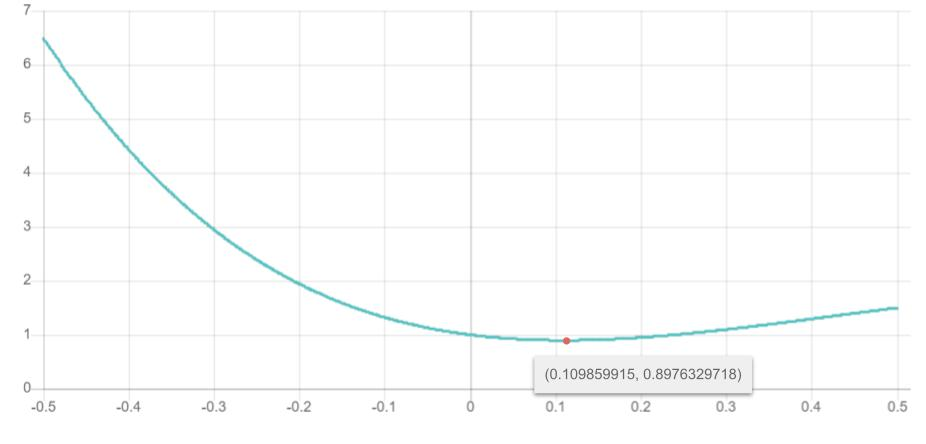
\includegraphics[scale=0.4]{figures/chart02}
\caption{Минимум}
\label{fig:universe}
\end{figure}


\section{Метод дихотомии}


% \newpage

\section{Реализация методов}
Вот сслыка на наш репозиторий:  \href{https://github.com/ddd127/metopt_labs}{metopt\_labs}


Реализация на языке Java конкретных методов:
\begin{itemize}
    \item \href{https://github.com/ddd127/metopt_labs/blob/master/src/main/java/com/example/metopt/math/minimization/impl/Dichotomy.java}{Метод дихотомии}
    \item \href{https://github.com/ddd127/metopt_labs/blob/master/src/main/java/com/example/metopt/math/minimization/impl/GoldenRatio.java}{Метод золотого сечения}
    \item \href{https://github.com/ddd127/metopt_labs/blob/master/src/main/java/com/example/metopt/math/minimization/impl/Fibonacci.java}{Метод Фиббоначи}
    \item \href{https://github.com/ddd127/metopt_labs/blob/master/src/main/java/com/example/metopt/math/minimization/impl/Parabola.java}{Метод параболл}
    \item \href{https://github.com/ddd127/metopt_labs/blob/master/src/main/java/com/example/metopt/math/minimization/impl/Brent.java}{Комбинированный метод Брента}
\end{itemize}

% \newpage

\section{Вывод}
Мы молодцы. Поставьте нам дофига баллов.


Кстати, вот ссылочка на сайт с нашими методами и графиками: \href{http://165.232.72.20:8080/}{dpk.com}


